%%%%%%%%%%%%%%%%%%%%%%%%%%%%%%%%%%%%%%%%%%%%%
%% Introdução à Cripotografia
%% Copyright 2006 Eliézio Batista de Oliveira
%%%%%%%%%%%%%%%%%%%%%%%%%%%%%%%%%%%%%%%%%%%%%

\chapter{Introdução à Criptografia}

A segurança provida pelo TLS é obtida através do uso de diversas 
técnicas criptográficas que, em conjunto, provêem os seguintes serviços de segurança 
conforme ilustrado na Figura~\vref{fig:crypto_blocks}, adaptada de \cite{Steffen}:

\begin{description}
	\item[Confidencialidade] -- É a garantia de que o conteúdo legível dos dados
	só estará acessível para as entidades autorizadas;
	\item[Integridade] -- É a garantia de que os dados não foram modificados inadvertidamente;
	\item[Autenticidade] -- É a garantia sobre a identidade da origem da informação\footnote{Vide
							\cite[seção~1.1]{hac} para uma definição mais ampla desse serviço.}.
\end{description}

Apresentaremos a seguir uma conceituação básica de cada uma dessas ferramentas.
Para uma introdução mais completa recomendamos o texto \emph{``Handbook of Applied Cryptography''} \cite{hac}.

\begin{figure}[htbp]
    \centering
		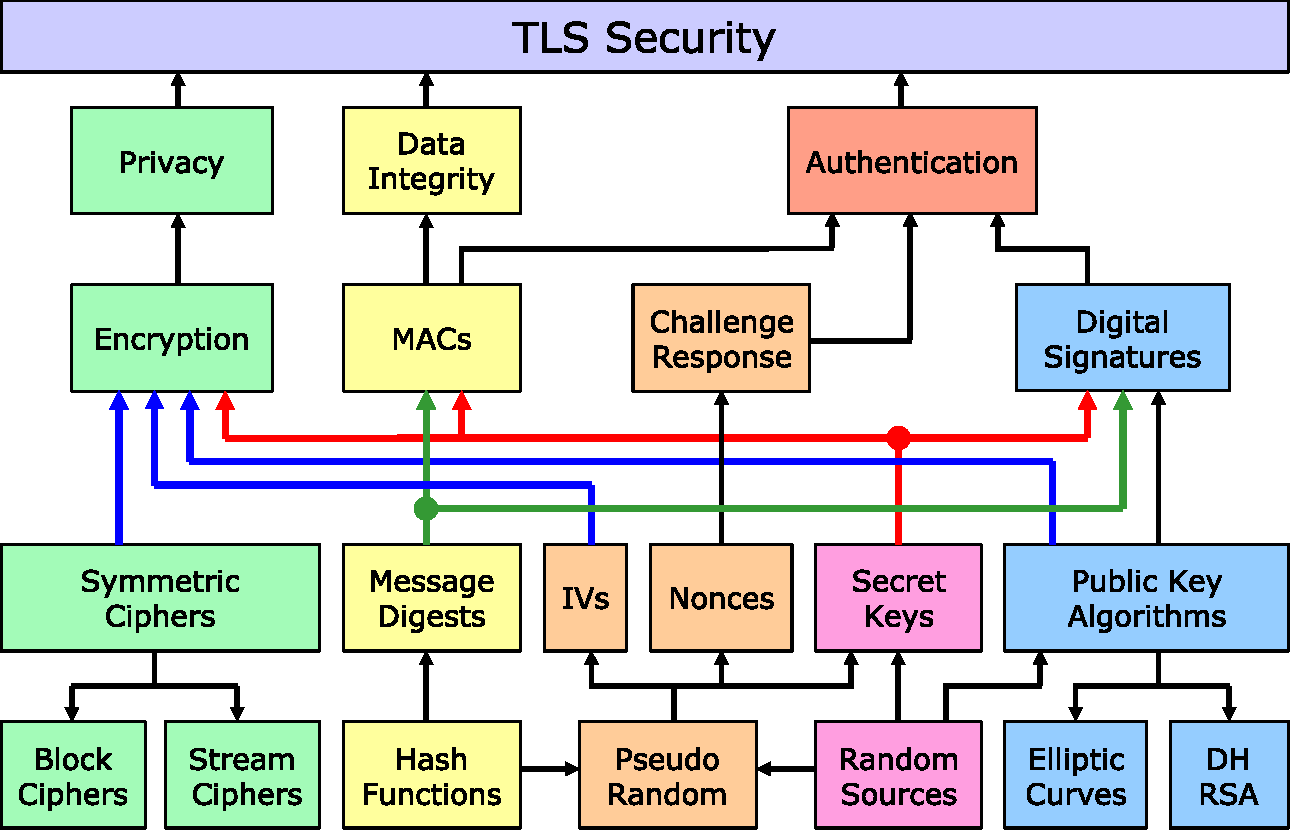
\includegraphics[width=\textwidth]{fig/crypto_blocks}
    \caption{Ferramentas criptográficas e suas inter-correlações}
    \label{fig:crypto_blocks}
\end{figure}

Como ainda não há um consenso na tradução para português de alguns termos 
básicos em criptografia, arbitramos pela seguinte terminologia nesse 
documento:

\begin{center}
    \begin{tabular}{@{}ll@{}} \toprule
	\tm{Inglês} & \tm{Português} \\ \midrule
encryption & cifragem \\
decryption & decifragem \\
cipher & cifrador \\
plaintext & mensagem ou texto legível \\
ciphertext & texto cifrado \\ \bottomrule
    \end{tabular}
\end{center}

Nas descrições dos algoritmos empregaremos a simbologia expressa na Tabela~\vref{tab:simbologiaAlgoritmos}.

\begin{table}[htbp]
	\centering
		\caption{Simbologia usada nas definições dos algoritmos}
		\begin{tabular}{@{}cl@{}} \toprule
		\tm{Símbolo} & \tm{Significado} \\ \midrule
		$m$ 						& Texto legível ou mensagem. \\
		$c$							& Texto cifrado. \\
		$h, i, r, s, v$				& Outros resultados/textos. \\
		\textsf{A} 					& Entidade origem. \\
		\textsf{B} 					& Entidade destino. \\
		$D, E, H, I, S, V$ 			& Funções/transformações. \\
		$\delta, \varepsilon, \kappa$ 	& Chaves criptográficas. \\
		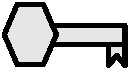
\includegraphics[scale=0.5]{fig/secret_key} & Chave secreta ($\kappa$). \\
		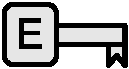
\includegraphics[scale=0.5]{fig/public_key} & Chave pública ($\delta$) da entidade ``E''. \\
		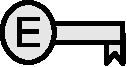
\includegraphics[scale=0.5]{fig/private_key} & Chave privada ($\varepsilon$) da entidade ``E''. \\ \bottomrule
		\end{tabular}
	\label{tab:simbologiaAlgoritmos}
\end{table}

\section{Funções de \emph{Hash} (resumo criptográfico)}

Uma Função de \emph{Hash} $H$ retorna, para uma mensagem $m$ de tamanho arbitrário 
qualquer, uma seqüência de bytes $h$ de tamanho fixo, chamada valor de \emph{hash} ou 
resumo criptográfico. Mais precisamente:
\[ h = H(m) \]
%Uma Função de \emph{Hash} criptograficamente segura deve apresentar as
%seguintes propriedades:

%\begin{description}
%    \item[Unidirecional] -- Encontrar $m = H^{-1}(h)$ deve ser
%    computacionalmente impraticável;
%    \item[Fracamente Livre de Colisões] -- Dada uma mensagem $m_1$, encontrar
%    $m_2$ diferente de $m_1$ tal que $H(m_1) = H(m_2)$ deve ser computacionalmente
%    impraticável;
%    \item[Fortemente Livre de Colisões] -- Encontrar $m_1$ e $m_2$ quaisquer
%    tal que $H(m_1) = H(m_2)$ deve ser computacionalmente impraticável.
%\end{description}
Dentre as diversas funções de \emph{Hash} existentes, o TLS limita-se aos algoritmos \acs{MD5} \cite{rfc_md5} e 
\acs{SHA1} \cite{fips_sha1}, cujos resumos são de 16 e 20 bytes respectivamente.

O valor de \emph{hash} quando representa a mensagem da qual derivou é chamado
de \emph{message digest}.

\section{Algoritmos de Chave Secreta}

Os algoritmos de chave secreta (\aclp{SKA} ou \acsp{SKA}) se caracterizam pela utilização de uma mesma chave para as 
operações complementares (cifrar/decifrar ou assinar/verificar).

A segura utilização destes algoritmos demanda, entretanto, pela solução de três problemas intrínsecos:

\begin{enumerate}
\item A distribuição confidencial da chave secreta entre duas entidades que precisa ser
efetuada \emph{a priori} por (outro) canal seguro;
\item O crescimento exponencial, da ordem de $O(n^2)$\footnote{A rigor: 
$\lim_{n \to \infty} \frac{n (n - 1)}{2} = n^2$},
da quantidade de chaves em função do número de entidades envolvidas ($n$)\footnote{Assumindo 
que será utilizada uma chave única para cada par de entidades.};
\item Como a sigilosidade de uma chave secreta decai na medida em que aumenta a sua exposição, torna-se
imperativo portanto que esta chave secreta tenha um curto ciclo de vida, requisito este difícil de 
ser atendido, considerando-se os dois problemas citados acima.
\end{enumerate}

No TLS, assim como em outros criptossistemas, esses problemas são resolvidos com o uso de
algoritmos de chave pública (ver seção~\ref{sec:pk}).

\subsection{\acl{MAC}}

O código de autenticação de mensagem (\acs{MAC}), também chamado de \ac{MIC},
é uma especialidade de resumo criptográfico computado em função
da mensagem $m$ e de uma chave secreta $\kappa$. A autenticidade da origem e a
integridade da mensagem podem ser comprovadas pelo destinatário usando-se a
mesma chave $\kappa$, como ilustra a Figura~\vref{fig:sk_sign}, na qual o
algoritmo de MAC/MIC está simbolizado pela função $I$ e o resumo por $i$.

\begin{figure}[htbp]
	\centering
		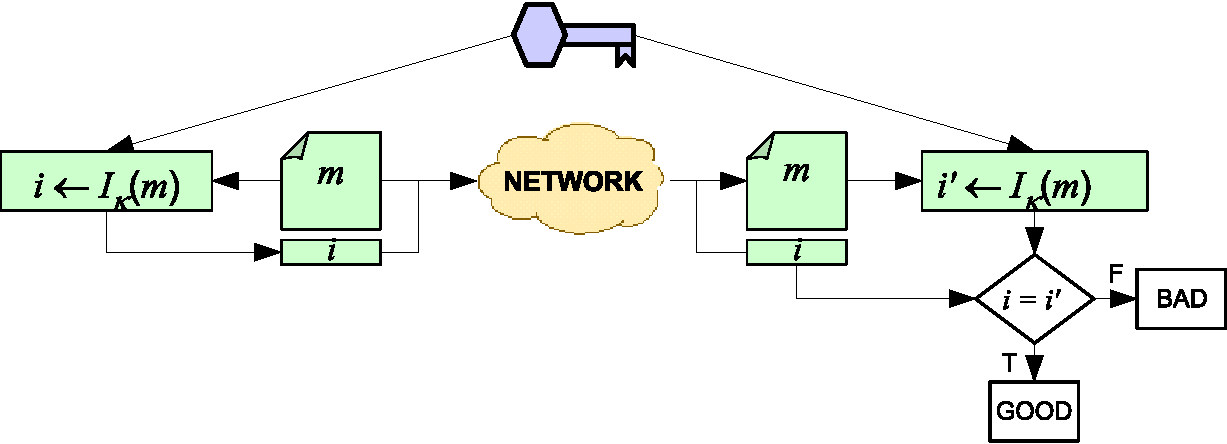
\includegraphics[scale=0.7]{fig/sk_sign}
	\caption{Geração e validação do MAC}
	\label{fig:sk_sign}
\end{figure}

Dentre os diversos tipos de \acs{MAC} já elaborados, o único
utilizado no TLS é o baseado em funções \emph{Hash}, mais precisamente o \ac{HMAC}
especificado em \cite{rfc_hmac} e que pode ser resumido na seguinte equação:
\[ i = HMAC_\kappa(H,m) = H(\kappa \oplus \mathtt{opad} \;\|\; H(\kappa \oplus \mathtt{ipad} \;\|\; m)) \]
onde:

\begin{tabular}{@{}rp{13cm}@{}}
$H(a)$		& Uma função de \emph{Hash} qualquer aplicada à seqüência $a$.
		  		  No caso do TLS, $H$ está limitado a \acs{MD5} ou \acs{SHA1}. \\
\addlinespace
$\kappa$	& Chave secreta com 64 bytes completada com zeros à direita. \\
\addlinespace
$\|$		& Operador de concatenação de seqüências. \\
\addlinespace
$\oplus$	& Operador binário OU-Exclusivo. \\
\addlinespace
$\mathtt{ipad}$ & O byte \texttt{0x36} repetido 64 vezes. \\
\addlinespace
$\mathtt{opad}$ & O byte \texttt{0x5C} repetido 64 vezes. \\
\end{tabular}

\subsection{Cifradores Simétricos}

Os cifradores simétricos utilizam a mesma chave $\kappa$ para o processo de cifragem ($E_\kappa$) 
e decifragem ($D_\kappa \equiv E_\kappa^{-1}$), conforme ilustra a Figura \vref{fig:sk_encryption}.

	\begin{figure}[htbp]
		\centering
			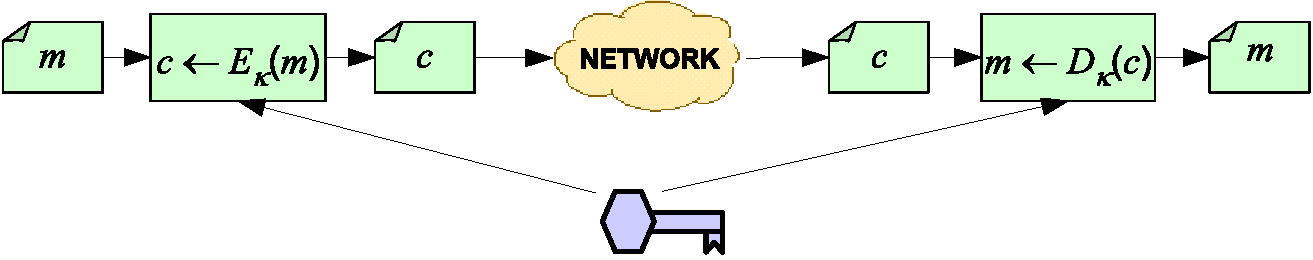
\includegraphics[scale=0.7]{fig/sk_cipher}
		\caption{Cifragem e decifragem usando SKA}
		\label{fig:sk_encryption}
	\end{figure}

Cifradores simétricos são normalmente classificados em seqüenciais
(\emph{stream ciphers}), que cifram/decifram um byte por vez, ou cifradores de
bloco (\emph{block ciphers}), que atuam sobre blocos de tamanho fixo,
usualmente 8 ou 16 bytes.

Dentre os cifradores simétricos oficialmente suportados pelo TLS, o único 
seqüencial é o RC4 \cite{rfc_rc4}. Os demais cifradores (de bloco) relacionados na norma são 
DES \cite{fips_des}, Triple-DES \cite{ansi_3des}, RC2 \cite{rfc_rc2} e IDEA \cite{idea}, que usam blocos de 8 bytes.

\section{Algoritmos de Chave Pública}
\label{sec:pk}

Os algoritmos de chave pública (\aclp{PKA} ou \acsp{PKA}) usam um par de chaves
matematicamente complementares, sendo uma delas tornada pública (doravante denotada por $\delta$) 
e a outra, chamada chave privada (simbolizada por $\varepsilon$), que deve ser conhecida apenas pela entidade
proprietária.

Esses algoritmos apresentam uma solução simples e revolucionária para o problema de distribuição de chaves, 
já que as chaves públicas não precisam trafegar por canais confidenciais. No entanto, a autenticidade da
origem das chaves e a integridade destas precisam estar asseguradas (ver seção \ref{sec:certs}).

Como é necessário distribuir apenas uma chave por entidade, os \acsp{PKA} estão naturalmente isentos do
segundo problema apresentado pelos \acsp{SKA}, já que o crescimento da quantidade de chaves é linear.

Em função de sua maior complexidade computacional, os \acsp{PKA} são tipicamente 10.000 vezes mais lentos
que os \acsp{SKA}. O TLS emprega então um criptossistema híbrido
onde os \acsp{SKA} são usados para os serviços de confidencialidade e integridade, com chaves secretas dinâmicas
estabelecidas através de \acsp{PKA}, que são também empregados para o serviço de autenticidade da origem e
assinatura digital.

Os \acsp{PKA} são tradicionalmente classificados conforme as seguintes propriedades~\cite{pki_book}:
cifragem , assinatura digital e estabelecimento de chave. 

\subsection{Cifragem}

Quando é reversível, ou seja, as duas transformações (denotadas por $E$ e $D$) são inversas entre si.

\begin{figure}[htbp]
	\centering
		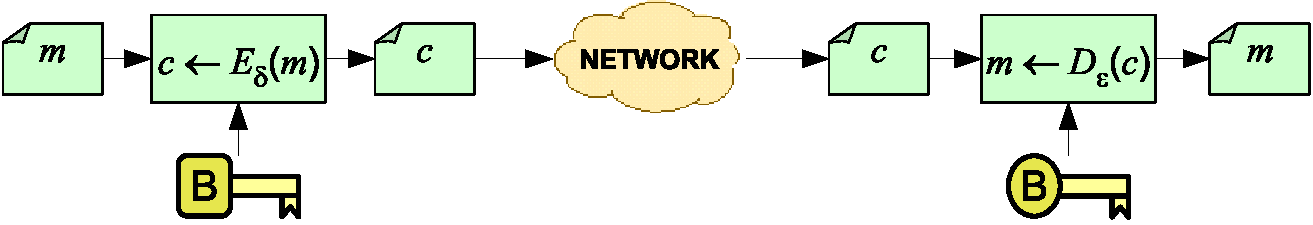
\includegraphics[scale=0.7]{fig/pk_cipher}
	\caption{Cifragem e decifragem com PKA}
	\label{fig:pk_encryption}
\end{figure}

O único algoritmo reversível oficializado na norma é o \acs{RSA} \cite{rsa}.

\subsection{Assinatura Digital}

Quando a sua chave privada pode ser utilizada por uma transformação $S_\varepsilon$
para a geração de um resumo especial (a ``assinatura'') 
a partir da texto legível. Este resumo será usado pela entidade destino que, com o uso da chave pública
da entidade origem e da função complementar $V_\delta$, poderá comprovar 
autenticidade e integridade da mensagem recebida.

\begin{figure}[htbp]
	\centering
		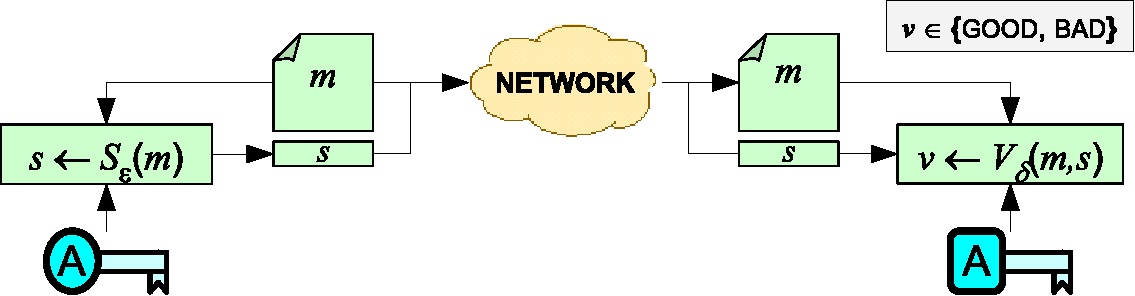
\includegraphics[scale=0.7]{fig/pk_sign}
	\caption{Assinatura Digital com PKA}
	\label{fig:pk_sign}
\end{figure}

A norma TLS especifica os algoritmos \ac{DSS} \cite{fips_dss} e o \acs{RSA} que, por ser reversível, pode ser 
usado aplicando-se as seguintes relações de equivalência:
\begin{eqnarray}
S_\varepsilon(m) & \equiv & E_\varepsilon(H(m)) \nonumber \\
V_\delta(m,s) & \equiv & D_\delta(s) \stackrel{?}{=} H(m) \nonumber
\end{eqnarray}

\subsection{Estabelecimento de Chave}

Quando o \acs{PKA} pode ser usado para a criação de um protocolo que permite o
compartilhamento de uma chave secreta entre as duas entidades participantes,
mas ainda assim confidencial. Existem dois métodos para este fim:
\begin{description}
	\item[Transferência] -- Uma das entidades é responsável pela geração da chave secreta que
	é enviada para a outra entidade após ser cifrada com chave pública desta, garantindo assim a
	confidencialidade da transferência.
	O PKA utilizado nesse caso deve ser obviamente reversível, como por exemplo o \acs{RSA}.
	\item[Comum Acordo] -- As duas entidades contribuem conjuntamente para a geração da chave secreta utilizando
	somente parâmetros criptográficos públicos, incluindo as chaves públicas de ambas as entidades.
	O \ac{DH} \cite{dh76} é um exemplo típico de algoritmo dessa categoria.
\end{description}

\section{Certificados Digitais}
\label{sec:certs}

No TLS todas as chaves públicas (PKs) devem ser armazenadas e distribuídas em certificados digitais
segundo o formato \acs{ITUT} X.509 versão 3 \cite{rfc_x509}. A principal finalidade de um
certificado é vincular uma chave pública à uma entidade final, conhecedora da respectiva
chave privada, e identificada por um nome universalmente único, denominado \acf{DN}.

A confiança na veracidade dessa associação é garantida pela assinatura digital emitida
por uma entidade confiável \emph{a priori}, chamada Autoridade Certificadora ou \ac{CA}.

Um certificado contém basicamente as seguintes informações:

\begin{itemize}
	\item DN da entidade final;
	\item PK correspondente com todos os seus parâmetros criptográficos necessários,
	junto com uma identificação do algoritmo (\acs{RSA} ou \acs{DSS});
	\item Período de validade;
	\item DN da CA emissora;
	\item Assinatura digital emitida pela \acs{CA}.
\end{itemize}

Um certificado contém também a definição sobre a política de utilização da PK nele contida,
se esta pode ou não ser utilizada para assinar outros certificados.

Quanto à política de utilização da sua PK e o tipo de assinatura do seu certificado,
as entidades são normalmente classificadas em três categorias:

\begin{center}
	\begin{tabular}{@{}lp{6cm}p{5cm}@{}} \toprule
		\tm{Tipo de} & \tm{Uso da PK}  	& \tm{Assinatura do} \\
		\tm{Entidade}&					& \tm{seu certificado} \\ \midrule
		Entidade final & Pode ser usada para qualquer propósito
						 \underline{exceto} para a assinatura digital. & Assinado por uma CA. \\
		CA Intermediária & Somente para a assinatura digital de outros certificados & Assinado por outra CA. \\
		CA Raiz			 & Idem & Auto-assinado. \\ \bottomrule
	\end{tabular}
\end{center}

A seqüência de certificados:
\[ C_0, C_1, C_2, \ldots, C_n \]

onde:

\begin{center}
	\begin{tabular}{@{}rl@{}}
		$C_0$ & Certificado da CA raiz, ou seja, auto-assinado. \\
		$C_1,\ldots,C_{n-1}$ & Certificados das CAs Intermediárias. \\
		$C_n$ & Certificado da entidade final. \\
	\end{tabular}
\end{center}

é chamada caminho de certificação (\emph{``Certification Path''}) da entidade final associada ao certificado $C_n$.
